\documentclass{memoir}

% I know, I know, I should use memoirs proper page things
\usepackage[cm]{fullpage}

\usepackage{tikz}
\usepackage{gurps}
\usepackage{times}
\usepackage{xparse}

\usepackage{gurps-npccard}

\setsecnumdepth{chapter}

\begin{document}

\section{Debbie Dyers}
\label{sec:debbie-dyers}
 
\begin{character*}[Debbie Dyers]
  \characterpicture{default.png}
  \ST{11} \DX{13} \IQ{12} \HT{12}
  \Will{15}

  \DR{15}

  \levelledadvantage{Hard to Kill}{2}
  \advantage{360\textsuperscript{o} Vision (Infrared only)}
  \advantage{Extra Attack}[25]
  \advantage{Signature Gear (Infrared sensor body suit)}

  \disadvantage{Vow (TODO figure out)}[-5]

  \skill{Guns (cordite pistol)}{16}
  \skill{Karate}{18}
\end{character*}

\printcharactercard{Debbie Dyers}
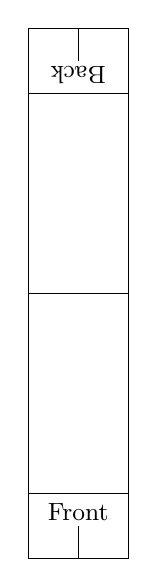
\begin{tikzpicture}[x=1in, y=1in]
  \draw (0,0) rectangle (0.5, -0.325);
  \draw (0.25,-0.325) -- (0.25,-0.1625);

  \draw (0,0) rectangle (0.5,2) node[pos=0.0,xshift=0.25in,anchor=north] {\small Front} node[pos=1.0,xshift=-0.25in,anchor=north,rotate=180] {\small Back};
  \draw (0,1) -- (0.5,1);

  \draw (0,2) rectangle (0.5, 2.325);
  \draw (0.25,2.325) -- (0.25,2.1625);
\end{tikzpicture}

Debbie Dyers is an independent bounty hunter who is legendary in the right
circles. She comes from a long line of hunters, the first of which was recorded
on earth who was allgegedly a `monster hunter' according to family folklore

An imposing figure at 6'2" with fiery red hair which extends to her shoulders.
She is usually sporting a trenchcoat which hides her extensive weaponry and
equipment.

Markedly against bio-enhancements, she has a special vest which gives her
360\textsuperscript{o} heat vision allowing her to aim at two (heat based)
targets at once.

% Little known sister to Leslie ``Trunchball'' Dyers
% (p.~\pageref{sec:lesl-trunchb-dyers}), Debbie is viewed as the `golden child' by her
% parents despite Trunchball's success in building \thecompany up from nothing.
% Debbie works for \emph{Dyers Independent}, a private bounty hunter company with
% one employee: Debbie.

\GCPrintCharacter[Debbie Dyers]

\end{document}

%%% Local Variables:
%%% mode: latex
%%% TeX-master: t
%%% End:
